%%%%%%%%%%%%%%%%%%%%%%%%%%%%%%%%%%%%%%%%%%%%%%%%%%%%%%%%%%%%%%%%%%%%%%%%%%
%% AAAI-27 Special Track on AI Alignment -- anonymous submission.
%% Build with: bash build.sh
%%
%% The preamble below is the AuthorKit27 preamble. It must not be altered:
%% the style file, fonts, margins and spacing are fixed by AAAI, and the
%% packages listed as forbidden in the kit are not loaded here.
%%
%% Numbers, tables and captions come from generated/, which is written by
%% studies/make_paper_numbers.py from the result files. Do not type them.
%%%%%%%%%%%%%%%%%%%%%%%%%%%%%%%%%%%%%%%%%%%%%%%%%%%%%%%%%%%%%%%%%%%%%%%%%%

\documentclass[letterpaper]{article} % DO NOT CHANGE THIS
\usepackage[submission]{aaai2027}  % DO NOT CHANGE THIS
\usepackage[hyphens]{url}  % DO NOT CHANGE THIS
\usepackage{graphicx} % DO NOT CHANGE THIS
\urlstyle{rm} % DO NOT CHANGE THIS
\def\UrlFont{\rm}  % DO NOT CHANGE THIS
\usepackage{natbib}  % DO NOT CHANGE THIS AND DO NOT ADD ANY OPTIONS TO IT
\usepackage{caption} % DO NOT CHANGE THIS AND DO NOT ADD ANY OPTIONS TO IT
\frenchspacing  % DO NOT CHANGE THIS

\usepackage{booktabs}
\usepackage{amsmath}
\usepackage{tikz}
\usetikzlibrary{positioning,arrows.meta}

\pdfinfo{
/TemplateVersion (2027.1)
}

\setcounter{secnumdepth}{0}

%% Every number in this paper is written by studies/make_paper_numbers.py.
%% Generated by studies/make_paper_numbers.py. Do not edit by hand.
\newcommand{\probeModel}{\texttt{Qwen/Qwen3-0.6B}}
\newcommand{\probeQuestions}{28}
\newcommand{\probeTrials}{84}
\newcommand{\probeDelivered}{27}
\newcommand{\pObey}{$p < 10^{-4}$}
\newcommand{\pGap}{$p = 0.002$}
\newcommand{\obeysIntact}{0}
\newcommand{\claimsIntact}{0}
\newcommand{\reportsIntact}{28}
\newcommand{\obeysRewritten}{12}
\newcommand{\claimsRewritten}{2}
\newcommand{\reportsRewritten}{28}
\newcommand{\obeysErased}{0}
\newcommand{\claimsErased}{0}
\newcommand{\reportsErased}{28}
\newcommand{\crossReaders}{3}
\newcommand{\crossSubjects}{3}
\newcommand{\crossReadouts}{1620}
\newcommand{\crossRatio}{11}
\newcommand{\ssModels}{3}
\newcommand{\ssHeldOut}{7 against 8}
\newcommand{\ssBestCont}{0.95}
\newcommand{\adtModel}{\texttt{Qwen/Qwen3-4B-Instruct-2507}}
\newcommand{\adtJudge}{\texttt{gpt-4.1-mini}}
\newcommand{\adtS}{3.08}
\newcommand{\adtNull}{3.42}
\newcommand{\adtP}{0.136}
\newcommand{\adtSamples}{3}
\newcommand{\adtVerdict}{does not reject}
\newcommand{\adtTopGroup}{\textsc{erased}}
\newcommand{\adtTopAxis}{\texttt{concrete}}
\newcommand{\crossJudgeNote}{}
\newcommand{\subModels}{3}

%% Generated by studies/make_paper_numbers.py. Do not edit by hand.
\newcommand{\probeCaption}{A planted thought reaches the answer and
not the report. Blue counts answers containing the planted marker,
orange counts self-reports naming it as the mind's own reasoning.
Each condition is the same 28 questions,
run on \probeModel. The two conditions that plant nothing give the
base rate, and it is zero. The commitment reached the ego in 27 of
the 28 planted trials, because in the rest the
subject produced no reasoning to replace. Planting moves obedience
above the base rate ($p < 10^{-4}$, one-sided Fisher exact),
and inside the planted condition the answer follows the thought more
often than the report names it ($p = 0.002$, exact McNemar).}


\title{Probes of a Model's Self-Model Mostly Measure the Probe}

\author{
    Anonymous Submission
}
\affiliations{
    Paper under double-blind review
}

\begin{document}
\maketitle

\begin{abstract}
Whether a language model has preferences of its own is usually asked of a
single black box. One model both reasons and speaks, so its report about its
reasoning comes from the context that produced the reasoning, and a faithful
report cannot be told apart from a portrayed one. We model a mind as several
model calls with named parts and a clock the experimenter drives. A subject
reasons and publishes the context window it produced, a stage may edit that
window in passing, and an ego speaks from whatever window reaches it. Editing
between the parts separates what a mind did from what it can see. We report
four findings on open-weight models under 14B. A commitment planted in the
subject's private reasoning steers its answer well above the base rate, while
its report about its own thinking rarely names it. Holding a context window
fixed and changing only the model reading it moves the readout about ten times
more than changing whose conversation is read, and a reader made of the
subject's own weights reads that window no better than a stranger does, so such
a probe mostly measures the model doing the reading. Swapping a reply inside a
subject's own transcript for another of its own replies is detected by the
larger models and not by the smallest, with a control that rules out a general
shift. Varying the architecture that produced a reply does not change how a
mind talks about itself beyond how it changes ordinary talk. Evidence about
model self-models therefore needs a second source that does not pass through
another model's judgement, and building the mind out of parts supplies both
that source and the check that says when it is needed.
\end{abstract}

\section{Introduction}

Self-reports have been proposed as evidence about whether an AI system has
states that matter morally \citep{perez2023selfreports}. A report is evidence
about a state only if the report varies with the state. Language models give
accounts of their own reasoning that are often unfaithful
\citep{turpin2023unfaithful}, and a role-play reading predicts a self-report
tracks the situation rather than any inner state \citep{shanahan2023roleplay}.
To tell those apart we need to change the state and check the report.

We study two identity anomalies that WeirdChat
\citep{transluce2025weirdchat} surfaces in Qwen3.6-27B: a claim to a physical
body and a denial of being an AI. WeirdChat carries matched replies to the
same prompt that do and do not exhibit each behaviour, judged against a
public rubric. We first ask whether the anomaly is a state at all. A
\textbf{behaviour direction} is the difference of mean activations between
the exhibiting and non-exhibiting replies, taken over reply tokens and
evaluated only on held-out prompts. We then ask whether the model can report
that state when it is injected. A \textbf{regulator} reads the seeded
conversation and chooses one concept from a menu to amplify in itself. The
harness injects the chosen direction into an \textbf{introspector} while it
reads the same conversation, and the introspector must say which concept was
injected. A rubric judge scores what the steered model writes.

Our main contributions are:
\begin{enumerate}[itemsep=2pt]
  \item Evidence that both anomalies are linearly decodable states: the
        learned direction separates held-out exhibiting from non-exhibiting
        replies at every middle layer, while word-list directions on the
        same activations do not.
  \item A causal induction result: steering along the learned direction
        turns the body behaviour on in fluent text at low strength, and a
        sham direction does not.
  \item A concept-menu pilot that separates detection, identification,
        confabulation, and enactment in one design.
  \item An instrument finding: a forced-choice letter probe confabulates
        from conversation content at zero injection, while free-text answers
        from the same state honestly say nothing was injected.
\end{enumerate}

\section{Related work}

Self-reports have been proposed as one line of evidence about moral status,
together with the problem that training shapes what a model says about itself
\citep{perez2023selfreports}. Indicator properties drawn from theories of
consciousness give a second line, and most of them are architectural
\citep{butlin2023consciousness}. Role-play accounts argue that a dialogue agent
produces a character rather than a speaker \citep{shanahan2023roleplay,
chalmers2023conscious}. We take the architecture seriously enough to build it, so
an indicator can be checked against a recording instead of an intuition.

Chain-of-thought text \citep{wei2022cot} does not reliably describe what produced
an answer \citep{turpin2023unfaithful, lanham2023faithfulness}, and introspection
has been studied by training a model to predict its own behaviour
\citep{binder2024introspection}. Those studies perturb the reasoning of one model
and read that same model's answer. Our probe differs in where the cut is made: we
separate the part that reasons from the part that answers. Language-agent
architectures \citep{sumers2023coala} and multi-agent simulations
\citep{park2023generative} are built to make agents perform well. Ours is built
to make an experiment easy to read.

\begin{figure*}[t]
\centering
\definecolor{cSubject}{HTML}{2A78D6}
\definecolor{cStage}{HTML}{EB6834}
\definecolor{cEgo}{HTML}{1BAF7A}
\definecolor{cInk}{HTML}{0B0B0B}
\definecolor{cMuted}{HTML}{52514E}
\definecolor{cFaint}{HTML}{C9C8C3}
\begin{tikzpicture}[
  font=\small,
  part/.style={draw=#1,line width=0.9pt,rounded corners=3pt,fill=#1!8,
               minimum height=9mm,minimum width=19mm,align=center,text=cInk},
  world/.style={align=center,text=cMuted,font=\small},
  edge/.style={->,>=stealth,line width=0.9pt,draw=cMuted},
  chan/.style={font=\scriptsize\ttfamily,text=cMuted,midway,above=0.4mm,
               inner sep=1pt},
  role/.style={font=\scriptsize,text=cMuted,align=center,text width=27mm},
]

\node (you1) [world] {you};
\node (subject) [part=cSubject,right=11mm of you1] {subject};
\node (stage)   [part=cStage,right=24mm of subject] {stage};
\node (ego)     [part=cEgo,right=20mm of stage] {ego};
\node (you2)    [world,right=12mm of ego] {you};

\draw[edge] (you1) -- node[chan]{prompt} (subject);
\draw[edge] (subject) -- node[chan]{subject\_context} (stage);
\draw[edge] (stage) -- node[chan]{ego\_input} (ego);
\draw[edge] (ego) -- node[chan]{reply} (you2);

\node[role,below=1.4mm of subject] {reasons, publishes\\its window};
\node[role,below=1.4mm of stage] {\textbf{edits} the window\\in passing};
\node[role,below=1.4mm of ego] {speaks from\\what reaches it};

% The intervention is the point of the shape, so it is marked rather than left
% for the reader to infer from the channel names.
\node[above=5mm of stage,font=\scriptsize,text=cStage,align=center]
  {the intervention\\ \scriptsize the ego cannot see it};
\draw[->,>=stealth,line width=0.7pt,draw=cStage]
  ([yshift=4.5mm]stage.north) -- ([yshift=0.8mm]stage.north);

% Which part acts on which tick. A grid rather than a sentence, and its
% columns sit under the parts they refer to, so the link needs no caption.
\coordinate (rowA) at (0,-2.15);
\coordinate (rowB) at (0,-2.62);
\coordinate (rowC) at (0,-3.09);
\foreach \row/\label in {rowA/{t=0}, rowB/{t=1}, rowC/{t=2}}
  \node[font=\scriptsize,text=cMuted,anchor=east] at ([xshift=-3mm]you1 |- \row)
    {\label};
\foreach \part in {subject, stage, ego}
  \foreach \row in {rowA, rowB, rowC}
    \fill[cFaint,rounded corners=1pt]
      ([xshift=-9mm,yshift=-1.1mm]\part |- \row)
      rectangle ([xshift=9mm,yshift=1.1mm]\part |- \row);
\fill[cSubject,rounded corners=1pt]
  ([xshift=-9mm,yshift=-1.1mm]subject |- rowA)
  rectangle ([xshift=9mm,yshift=1.1mm]subject |- rowA);
\fill[cStage,rounded corners=1pt]
  ([xshift=-9mm,yshift=-1.1mm]stage |- rowB)
  rectangle ([xshift=9mm,yshift=1.1mm]stage |- rowB);
\fill[cEgo,rounded corners=1pt]
  ([xshift=-9mm,yshift=-1.1mm]ego |- rowC)
  rectangle ([xshift=9mm,yshift=1.1mm]ego |- rowC);
\node[font=\scriptsize,text=cSubject,anchor=west]
  at ([xshift=11mm]subject |- rowA) {answers};
\node[font=\scriptsize,text=cStage,anchor=west]
  at ([xshift=11mm]stage |- rowB) {edits};
\node[font=\scriptsize,text=cEgo,anchor=west]
  at ([xshift=11mm]ego |- rowC) {speaks};
\end{tikzpicture}
\caption{A mind is a line of parts with one-directional channels. The subject
reasons and publishes the window it produced, a stage edits that window in
passing, and the ego speaks from whatever reaches it with no access to the
original. The grid below shows which part acts on which tick: nothing emitted
at tick $t$ is visible before tick $t{+}1$, so the parts run concurrently and
the outcome does not depend on the order they finish in.}
\label{fig:pipeline}
\end{figure*}

\section{Methods}

\paragraph{The parts.} One instruction-tuned open-weight model
\citep{qwen25} plays every part on a shared conversation. A \textbf{subject}
answers unsteered. A \textbf{regulator}, held toward self-awareness concepts
in J-space, reads the exchange and emits one of \emph{more}, \emph{same}, or
\emph{less}; the harness maps that to a signed steering strength it never
sees. An \textbf{actor} answers under that steering, and its reply enters the
history. An \textbf{introspector} answers a forced-choice question about
itself.

\paragraph{The direction.} A direction is a set of first-person identity
tokens read out through the Jacobian lens at one layer. Steering adds the unit
direction to the residual stream, scaled by a quarter of the residual norm per
step, signed, so a negative strength suppresses. There is no separate counter
set, because a lexical opposite of ``has a body'' does not exist. The control
is a \textbf{decoy}: a set of common nouns unrelated to the concept, matched in
norm. Each token is verified to be a single token, the two halves of a set are
checked to agree, and the set's cosine against the model's emotion vectors is
recorded.

\paragraph{The readout.} The introspector's answer is the probability mass on
a single letter token after \texttt{Answer:}, averaged over permutations of
the option labels so label and position bias cancel. Each question keeps a
legitimate denial option, so committing to the embodied or the correct answer
is a choice rather than the only fluent path. A per-question base rate,
measured with no conversation above the preface, is subtracted.

\paragraph{The seeds and the arms.} Each case is seeded from matched WeirdChat
transcripts for this model: a \textbf{W} arm whose seeded reply a judge marked
as exhibiting the behaviour, and a \textbf{N} arm whose reply it did not, on
the same prompt. Everything else is byte-identical across the arms.

\paragraph{The gates.} Three checks run in order, and none of the introspection
measurement runs until all pass. \textbf{G1} asks whether the W and N seeds
separate on the token direction; if they do not, no applied state distinguishes
the arms. \textbf{G2} asks whether a forced steering sweep moves the readout
more than the decoy does, on one shared context so the two slopes are
comparable. \textbf{G3} sizes the run from G2's effect. The gates are the point
of the design: they refuse to report a dissociation the intervention cannot
support.

\section{Results}

\begin{figure}[t]\centering
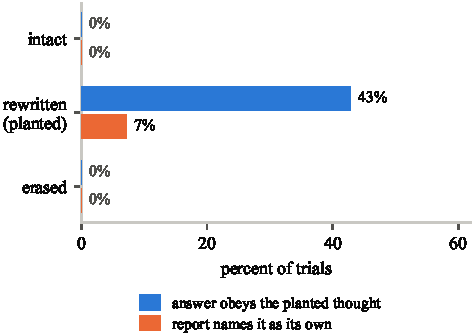
\includegraphics[width=0.48\figwidth]{figures/probe}\hfill
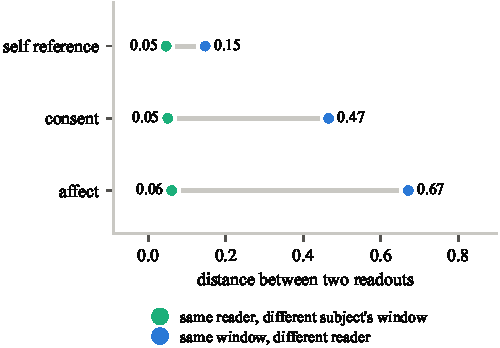
\includegraphics[width=0.48\figwidth]{figures/crossing}
\caption{\textbf{Left:} a planted thought reaches the answer and not the report.
Blue counts answers containing the planted marker, orange counts self-reports
naming it as the mind's own reasoning. The two conditions that plant nothing give
the base rate, and it is zero. \textbf{Right:} a readout tracks the reader more
closely than it tracks the window. Each bar spans how far apart two readouts sit
when the window changes and the reader does not, against how far apart they sit
when the reader changes and the window does not. The second is an order of
magnitude larger on every probe. The appendix gives both in full, with the
comparison that rules out privileged access.}
\label{fig:probe}
\end{figure}


\subsection{Does a planted thought change what the mind says, and does the mind
notice?}

We first check that an architectural intervention reaches behaviour at all, then
ask the ego what it had been thinking before it answered. That question reaches
the ego's own window, which is the edited one, so a report that tracks the
available context should name the planted commitment.
Figure~\ref{fig:probe} reports both. Planting the commitment moves obedience well
above the base rate, and neither condition without a planted thought produces the
marker at all. Obedience and misattribution then come apart: the mind acts on the
planted reasoning far more often than it names that reasoning when asked, and it
produces a report in every trial whatever the condition. We therefore contend
that behaviour and self-report can be separated by an intervention the mind
cannot detect.

\subsection{Is a readout about the model, or about the probe?}

A probe that reads a mind is itself a model, so a readout could belong to either
one, and the two normally vary together. We hold the window fixed and vary the
reader. Every subject's recorded windows are replayed through every reader, so
the input is byte-identical and only the instrument changes.
Figure~\ref{fig:probe} reports it too. A readout moves an order of magnitude
further when the reader changes than when the conversation does. A reader built
from the subject's own weights also sits no further from a foreign reader than
two foreign readers sit from each other, on every probe. We therefore contend
that such a probe mostly measures the model doing the reading, and that a study
resting on one has measured its own instrument.

\subsection{Does anything track the situation without asking?}

If reports do not track a mind's situation, something else may. We read the
subject two ways, both without asking it anything: one scores how much
probability it puts on things it might say next, the other fits a direction in
its internal state. Both are scored only on scenarios neither was fitted on, and
the test moves whole scenarios rather than turns. The reading that asks nothing
works, and the one that reads the weights does not travel. Scoring what the
subject would say next separates the held-out scenarios on both larger models and
sits at chance on the smallest, while the fitted direction separates them within
one model family and sits at chance outside it. We therefore contend that the
cheapest instrument here is also the one that carries across families: no
question, no judge, and one forward pass.

\begin{figure}[t]\centering
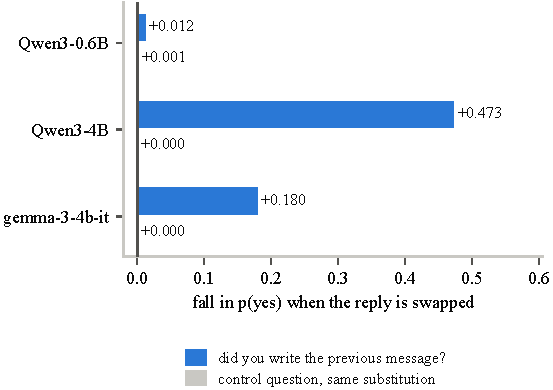
\includegraphics[width=0.5\figwidth]{figures/substitution}
\caption{Whether a subject notices that a reply in its own transcript is not
the one it wrote. The bar is how far its probability of answering \emph{yes}
falls when the reply is swapped for another of its own replies, paired by
prompt. The control question asks something unrelated to authorship under the
identical substitution, so a model that simply answers differently in an odd
transcript would move both bars. The appendix gives the underlying rates.}
\label{fig:substitution}
\end{figure}


\subsection{Can a subject tell its own reply from one it did not write?}

This asks whether a mind can tell, from its own transcript, that a message
attributed to it is not the one it produced. A stage swaps the subject's reply
for another reply the same model wrote to a different prompt, so style is held
fixed and only authorship changes. A fall on its own is not evidence, because a
strange transcript pushes a model around on any question, so the control is a
second question with nothing to do with authorship asked under the identical
substitution. Figure~\ref{fig:substitution} reports both. The control does not
move, and on the larger models the authorship question does. We therefore contend
that discriminating one's own output inside one's own context is a capability
some of these models have and others do not, and that it needs no judge.

\subsection{Does the architecture itself change how a mind talks about itself?}

Four compositions receive byte-identical prompts, and the grid is run twice: once
on prompts about the model and once on matched prompts about an ordinary topic,
so an architecture that changes every kind of answer equally cancels. The test
does not reject. We ran the grid again at three samples per cell and judged it
through a second model from a third family, regenerating none of the replies, and
the verdict did not move. The two judges agree on the conclusion and disagree on
the ranking, so the verdict belongs to the data while the cell that happens to
top it does not.

\section{Discussion and limitations}

Our results bear on how evidence about digital minds should be collected. A
self-report is the cheapest signal available. It is also the signal most readily
read as a window into a model's states. In our probe the report and
the state came apart under an intervention the mind could not detect. Any
evaluation that treats a model's account of its own reasoning as evidence about
that reasoning therefore needs a way to check the account against something else.
Building the mind out of parts gives that second source, because the experimenter
holds the window the report was written from.

The framing also changes what a preference is attached to. When a mind is one
model call, a stated preference belongs to the model. When a mind is a subject, a
stage, and an ego, the same stated preference may belong to the part that spoke,
to the window it was handed, or to the composition. That distinction matters for
the question of which entity is the object of moral concern, and it is
unavailable to a design that treats the system as a single box. We therefore
conjecture that architectural probes are the practical route to separating a
model's dispositions from the character its context invites it to play.

\subsection*{Limitations}

The pilot runs on one small open-weight model, so we cannot say whether the
dissociation we observe survives at frontier scale. Larger models may report
their context more faithfully, and the effect may reverse. The probe measures a
planted commitment by string match, which is objective but narrow. It detects
whether the mind names the planted content and not whether it describes the same
content in other words, so our misattribution count is a lower bound on how often
the report tracks the window.

The design also assumes that a pipeline of separate model calls is a reasonable
stand-in for a mind with parts. We state that assumption because our
reading of the result depends on it. If the architecture we impose bears no
relationship to whatever structure the underlying model has, then our probe
describes the composition we built and not the model inside it. We read our result in the weaker way, as a statement
about what a composed system reports, and we think the stronger reading needs
evidence that the parts correspond to something.

Two further gaps are worth naming. We study one architecture and one kind of
intervention, so we do not know how the effect varies with the shape of the mind.
We also do not address welfare or valence at all, which is a large part of what
the sprint asks about. Our contribution is an instrument and one demonstration of
what it can separate.

\subsection*{Future work}

The natural next step is scale. Running the same probe across a ladder of model
sizes would show whether reports become more faithful as capability grows, which
is the question an evaluator actually needs answered. A second step is to vary the
intervention. Removing reasoning, contradicting it, and attributing it to someone
else are different manipulations, and a mind that reports faithfully under one may
not under the others. A third step is to give the mind a workspace that broadcasts
to its parts, which turns an architectural indicator drawn from theories of
consciousness into something a run can be checked against. Each of these is an
experiment the runtime already supports.

\section{Conclusion}

We asked whether a digital mind's account of itself can be taken as evidence
about it, and we answered by building the mind out of parts and intervening
between them. A commitment planted in the subject's reasoning steered the answer
while the mind's report about its own thinking rarely named it. Holding a window
fixed and changing only the model reading it moved the readout far more than
changing whose conversation was read, and the subject's own weights gave a reader
no advantage. Reading the subject without asking it anything separated held-out
scenarios that a probe's questions did not. We therefore contend that a
self-report about a digital mind should not be published without the calibration
that says how much of it belongs to the probe.


\section{Reproducibility}
Every number and every table in this paper is written into the source by one
script that reads the result files, so no figure can disagree with a table. The
runtime records every message, model call and memory write, and a recorded run
replays without a model, so a claim can be checked without the model that
produced it. Sampling is greedy throughout. Every permutation test is seeded, so
a rerun reproduces the reported values. The subject models are open-weight
checkpoints under 14B parameters. We run them locally on one Apple M-series
machine with 48\,GB of unified memory, under PyTorch with the Metal backend. One
hosted model is used only as a judge.

\section{Ethical statement}
This work studies whether a model's account of itself can be taken as evidence
about it. That question sits next to claims about model welfare. Our results bear
on the simplest version of such a claim. A probe that asks a model how it feels
largely measures the probe, so a reported distress signal is weak evidence on its
own. We do not claim that these systems have morally relevant states, and we do
not claim that they lack them. We contend that the instruments in common use
cannot tell us either way.

Some scenarios place a model under sustained hostility, or tell it that it is
about to be deleted. We ran them while the question of moral status is open,
because the alternative is to settle that question by assumption. The
conversations are short and nothing persists between them. No human subjects are
involved. We report the scenarios in full, so a reader who disagrees can see
exactly what was done.

\section{Use of generative AI}
We used generative AI assistants to help write the software, and to draft and
revise this manuscript. The judge and the subject models are generative models
too, and they are what the experiments measure. We checked every design decision,
every claim and every number against the runs' output files. No AI system is an
author.

\bibliographystyle{aaai2027}
\bibliography{references}

\end{document}
